\documentclass{beamer}
\usepackage[utf8x]{inputenc}
\usepackage[ngerman]{babel}
\usepackage{amsmath}
\usepackage{amsfonts}
\usepackage{amssymb}
\usepackage{graphicx}
\usepackage{subfigure}
\author{Johannes Hackel\and Falco Prescher}
\title{WebSocket}

\usetheme{Ilmenau}
\useoutertheme{infolines}
\usecolortheme{rose}

\begin{document}

\begin{frame}
\titlepage
\end{frame}

\begin{frame}
\frametitle{Gliederung}
\tableofcontents
\end{frame}

\section{Definition}
\begin{frame}
\frametitle{Definition}
\end{frame}

\section{Warum?}
\begin{frame}
\frametitle{Warum?}

\begin{itemize}
\item immer mehr Anwendungen durch Webtechnologien
\item fehlende Echtzeit
\item vorher durch Polling/Long Polling
\item führt zu viel Overhead und Netzwerkauslastung
\end{itemize}

\end{frame}


\begin{frame}
\frametitle{Polling/Long Polling}
\begin{figure}
\subfigure{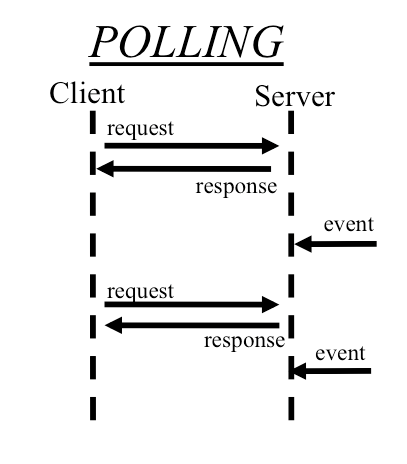
\includegraphics[width=5cm]{polling.png}}
\subfigure{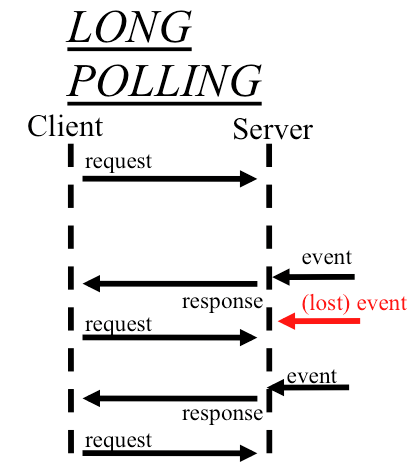
\includegraphics[width=5cm]{long_polling.png}}
\end{figure}
\end{frame}

\begin{frame}
\begin{figure}
\begin{center}
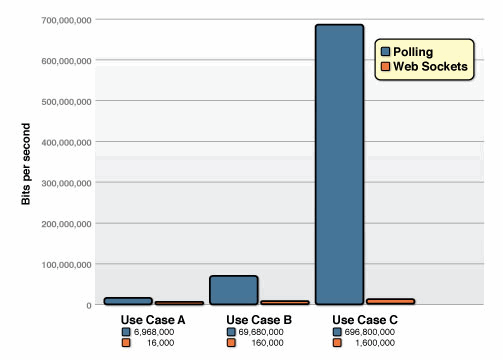
\includegraphics[width=12cm]{poll-ws-compare.png}
\end{center}
\end{figure}
\end{frame}

\section{Verwendungen}
\begin{frame}
\frametitle{Verwendungen}
\begin{itemize}
\item Facebook, Twitter
\item Chats
\item kollaborative Websites (etherpad)
\item Spiele auf HTML5-Basis
\end{itemize}
\end{frame}

\section{Bestandteile}

\subsection{Netzwerkprotokoll}
\begin{frame}
\frametitle{Bestandteile}
\framesubtitle{Netzwerkprotokoll}
\end{frame}

\subsection{Javascript Client-API}
\begin{frame}
\frametitle{Bestandteile}
\framesubtitle{Javascript Client-API}
\end{frame}

\section{Implementierungen/Technologien}
\begin{frame}
\frametitle{Implementierungen/Technologien}
\end{frame}

\section{Zusammenfassung}
\begin{frame}
\frametitle{Zusammenfassung}
\end{frame}

\section{Quellen}
\begin{frame}
\frametitle{Quellen}
\begin{itemize}
\item http://www.heise.de/developer/artikel/WebSocket-Annaeherung-an-Echtzeit-im-Web-1260189.html
\item http://www.websocket.org
\end{itemize}
\end{frame}

\end{document}